\section{Results and Discussion}
%Need to explain the experimental set up here. Omnidirectional camera, monarch platform. And motivating the experiments below. 
\dv{Need to identify one or two scenarios where the uncertainity will help us. Like two people standing close by and the robot not going in between them. In the other case with deterministic tracker, the robot should go in between them.}\\

For each of the scenarios described in section \ref{sec:scenarios}, we have compare the results obtained from the 1)basic navigation method, 2)deterministic human-aware navigation, 3)kmeans clustering human-aware navigation, 4)shifted means clustering human-aware navigation, 5)social cost convolution human-aware navigation for both FMM and DWA. 
Sample results from simulations for the case of static people, are also depicted in Figure ? for comparing the results of our simulations with reality.



%1. FMM + without uncertainity\\2. FMM + with uncertainity\\	2a. Convolution\\	2b. clustering\\3. DWA + without uncertainity\\4. DWA + with uncertainity\\	2a. Convolution\\	2b. clustering\\

%All these should have simulations and real robot experiments.\\


\subsection{Results}
\label{sec:results}

Figures
Tables of parameters


\begin{figure}[t!]
\centering
\subfloat[]{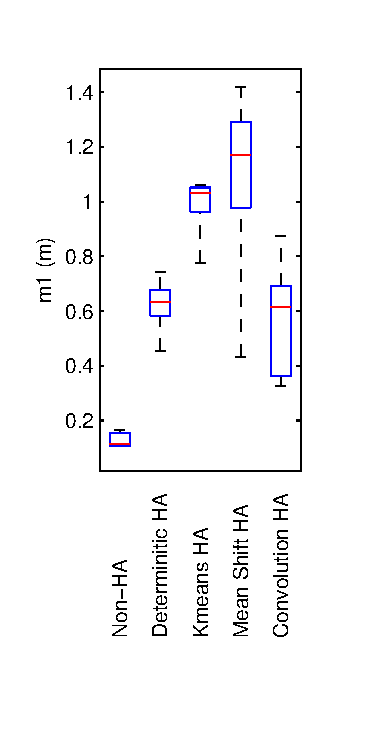
\includegraphics[width=0.152\textwidth]{pictures/m1.eps}\label{fig:1}}%
\hspace{0.1cm}
\subfloat[]{\includegraphics[width=0.153\textwidth]{pictures/m2.eps}\label{fig:2}}%
\hspace{0.1cm}
\subfloat[]{\includegraphics[width=0.153\textwidth]{pictures/m3.eps}\label{fig:3}}%
\hspace{0.1cm}
\subfloat[]{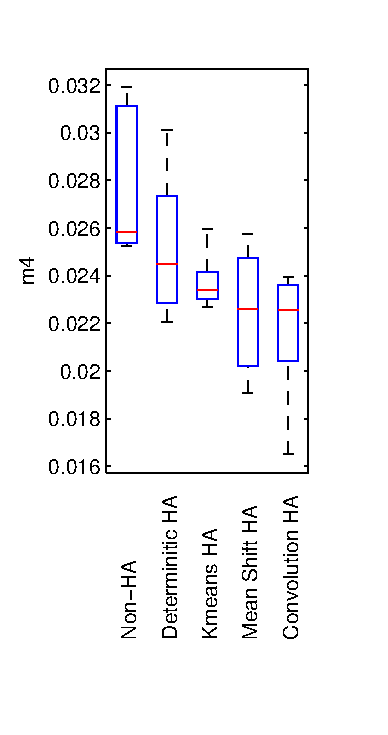
\includegraphics[width=0.153\textwidth]{pictures/m4.eps}\label{fig:2}}%
\hspace{0.1cm}
\subfloat[]{\includegraphics[width=0.153\textwidth]{pictures/m5.eps}\label{fig:3}}%

\caption{Boxplots for the three metrics acquired for STATIC SINGLE PERSON}
\label{fig:boxplots_singlePerson}
\end{figure}

\begin{figure}[t!]
\centering
\subfloat[]{\includegraphics[width=0.153\textwidth]{pictures/dy_m4.eps}\label{fig:2}}%
\hspace{0.1cm}
\subfloat[]{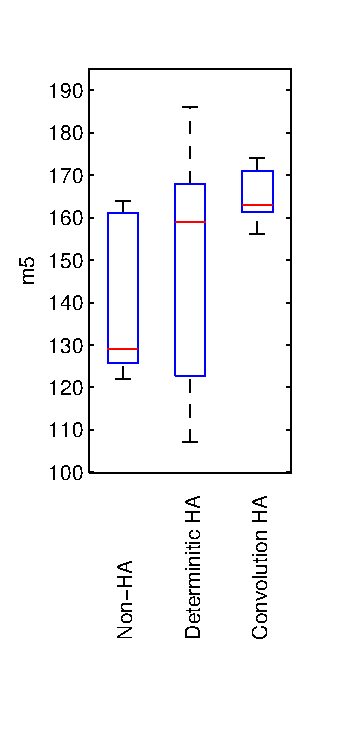
\includegraphics[width=0.153\textwidth]{pictures/dy_m5.eps}\label{fig:3}}%

\caption{Boxplots for the three metrics acquired for STATIC MOVING PERSON}
\label{fig:boxplots_singlePersonMov}
\end{figure}


\begin{figure}[t!]
\centering
\subfloat[]{\includegraphics[width=0.152\textwidth]{pictures/two_m1.eps}\label{fig:1}}%
\hspace{0.1cm}
\subfloat[]{\includegraphics[width=0.153\textwidth]{pictures/two_m2.eps}\label{fig:2}}%
\hspace{0.1cm}
\subfloat[]{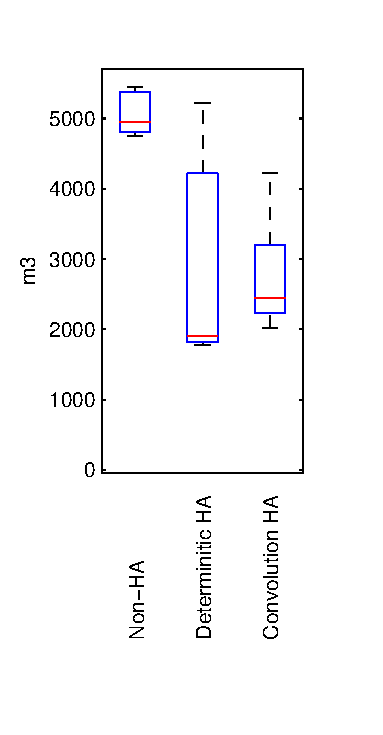
\includegraphics[width=0.153\textwidth]{pictures/two_m3.eps}\label{fig:3}}%
\hspace{0.1cm}
\subfloat[]{\includegraphics[width=0.153\textwidth]{pictures/two_m4.eps}\label{fig:2}}%
\hspace{0.1cm}
\subfloat[]{\includegraphics[width=0.153\textwidth]{pictures/two_m5.eps}\label{fig:3}}%
\hspace{0.1cm}
\subfloat[]{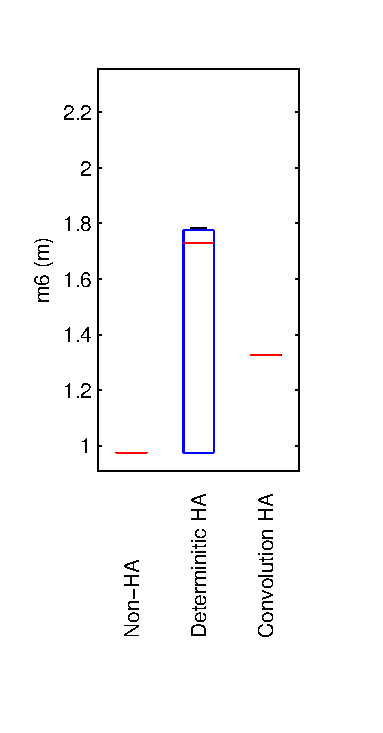
\includegraphics[width=0.153\textwidth]{pictures/two_m6.eps}\label{fig:3}}%

\caption{Boxplots for the three metrics acquired for 2 PERSONS STATIC}
\label{fig:boxplots_2people}
\end{figure}


\subsection{Discussion}
\label{sec:discussion}

Reasoning about the figures.

We expect to see improvements when applying FMM and more so when considering in uncertainty of perception. Convolution method given its higher flexibility and not requiring the number of people in the scenario is expected to give better results.

DWA cant make a noticeable difference in the trajectories, due to the tendency of the robot to take velocity candidate that are tangent to the planned path and small differences in the new positions of the robot that each candidate will cause. However, it does a good job of discarding velocity candidates that result in uncomfortable accelerations or speeds.


keans vs shifted : 
 More accurate and closer to reality based on our simulations and real collected data from the probabilistic tracker.